\author{Josef Stieg}

\section{Beschreibung}

\subsection{Grundfunktion}

Die innovative Online-Plattform \textit{Melius} bietet Nutzer:innen die Möglichkeit, professionelle und personalisierte Portfolios zu erstellen, die insbesondere im Bewerbungsprozess von großem Nutzen sind. Die Intention der Plattform besteht in der Simplifikation und Effektivierung des Bewerbungsprozesses. Dies wird erreicht, indem alle relevanten Informationen und Materialien an einem zentralen Ort gesammelt und übersichtlich dargestellt werden.

Die Plattform bietet drei Hauptkategorien, in denen Nutzer:innen ihre Informationen speichern und strukturieren können:

Der Lebenslauf bietet die Möglichkeit, klassische Daten wie Kontaktdaten, Ausbildung und Berufserfahrung einzugeben und übersichtlich aufzubereiten. Der integrierte Editor erlaubt die Gestaltung eines individuellen und professionellen Lebenslaufs, der sich nahtlos in das gesamte Portfolio einfügt.

Die Projektseite ermöglicht die Präsentation bisheriger Projekte. Die Möglichkeit der Integration visueller Elemente wie Bilder oder Screenshots erlaubt eine anschauliche Darstellung der Projekte. Für Nutzer:innen mit technischem Hintergrund besteht zudem die Option der direkten Integration von GitHub-Repositories. Dies erlaubt die authentische und nachvollziehbare Präsentation von Programmierprojekten oder anderen Softwareentwicklungen.

Die Seite "Kompetenzen" bietet die Möglichkeit, spezifische Fähigkeiten und Kompetenzen hervorzuheben, die für die angestrebte Position von Relevanz sind. Diesbezüglich besteht die Möglichkeit, die relevanten Fähigkeiten und sozialen Kompetenzen in einer übersichtlichen und klar strukturierten Form darzustellen.

\newpage

Ein besonderes Merkmal von \textit{Melius} ist die Integration und Präsentation aller Daten in einem einheitlichen, ästhetisch ansprechenden Format. Der zeitaufwändige Prozess der Zusammenführung verschiedener Dateien und Formate wie PDF-Lebensläufe, Portfolio-Dokumente oder Projektbilder manuell wird somit obsolet.

Ein weiteres herausragendes Merkmal der Plattform ist die Möglichkeit, das vollständige Portfolio unkompliziert über einen einzigen Link zu teilen. Dies ist insbesondere für Bewerberinnen und Bewerber von Vorteil, da sie sich nicht länger mit dem Anhängen umfangreicher Dateien oder der Überschreitung von E-Mail-Datenlimits befassen müssen. Der Link führt direkt zu einer eigenen, personalisierten Online-Präsenz, welche potenziellen Arbeitgeberinnen und Arbeitgebern einen unmittelbaren und umfassenden Überblick über die Qualifikationen und Erfahrungen der Bewerberinnen und Bewerber ermöglicht.
    
\begin{figure}[H]
    \centering
    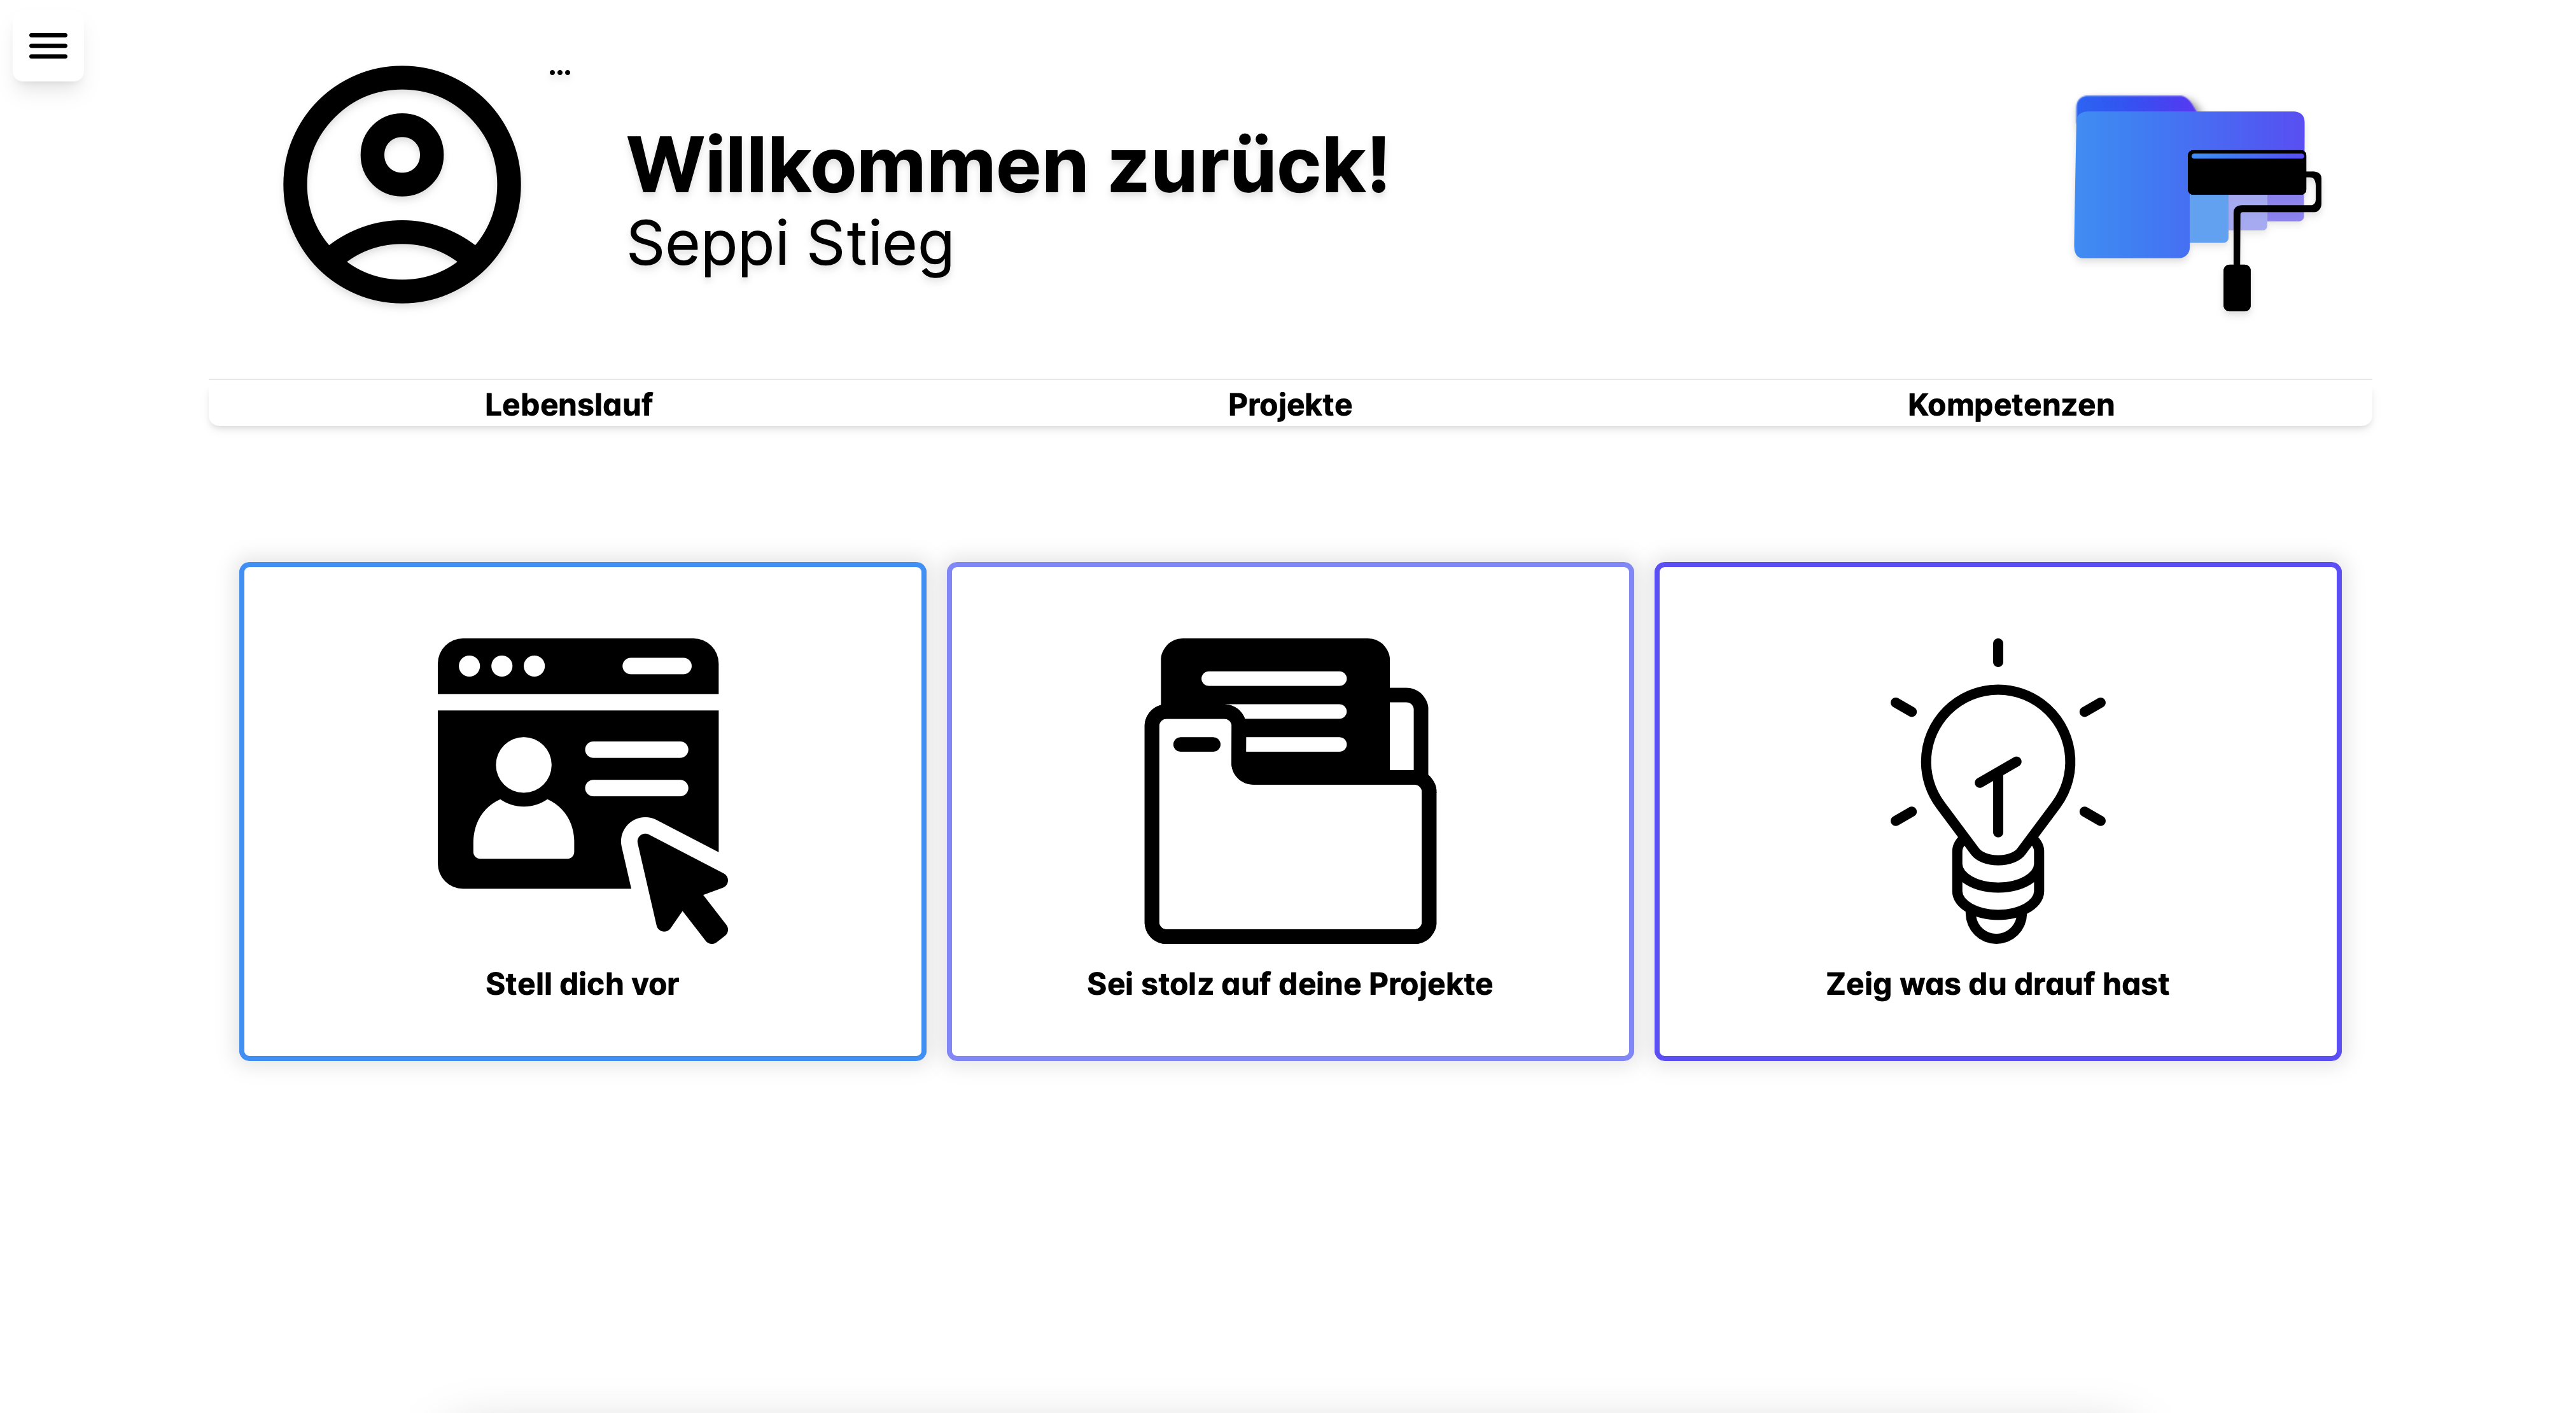
\includegraphics[scale=0.15]{pics/Einführung/Melius_HomePage.png}
    \caption{Abbildung der Melius Home Page}
    \label{fig:int:cv}
\end{figure}

\begin{figure}[H]
    \centering
    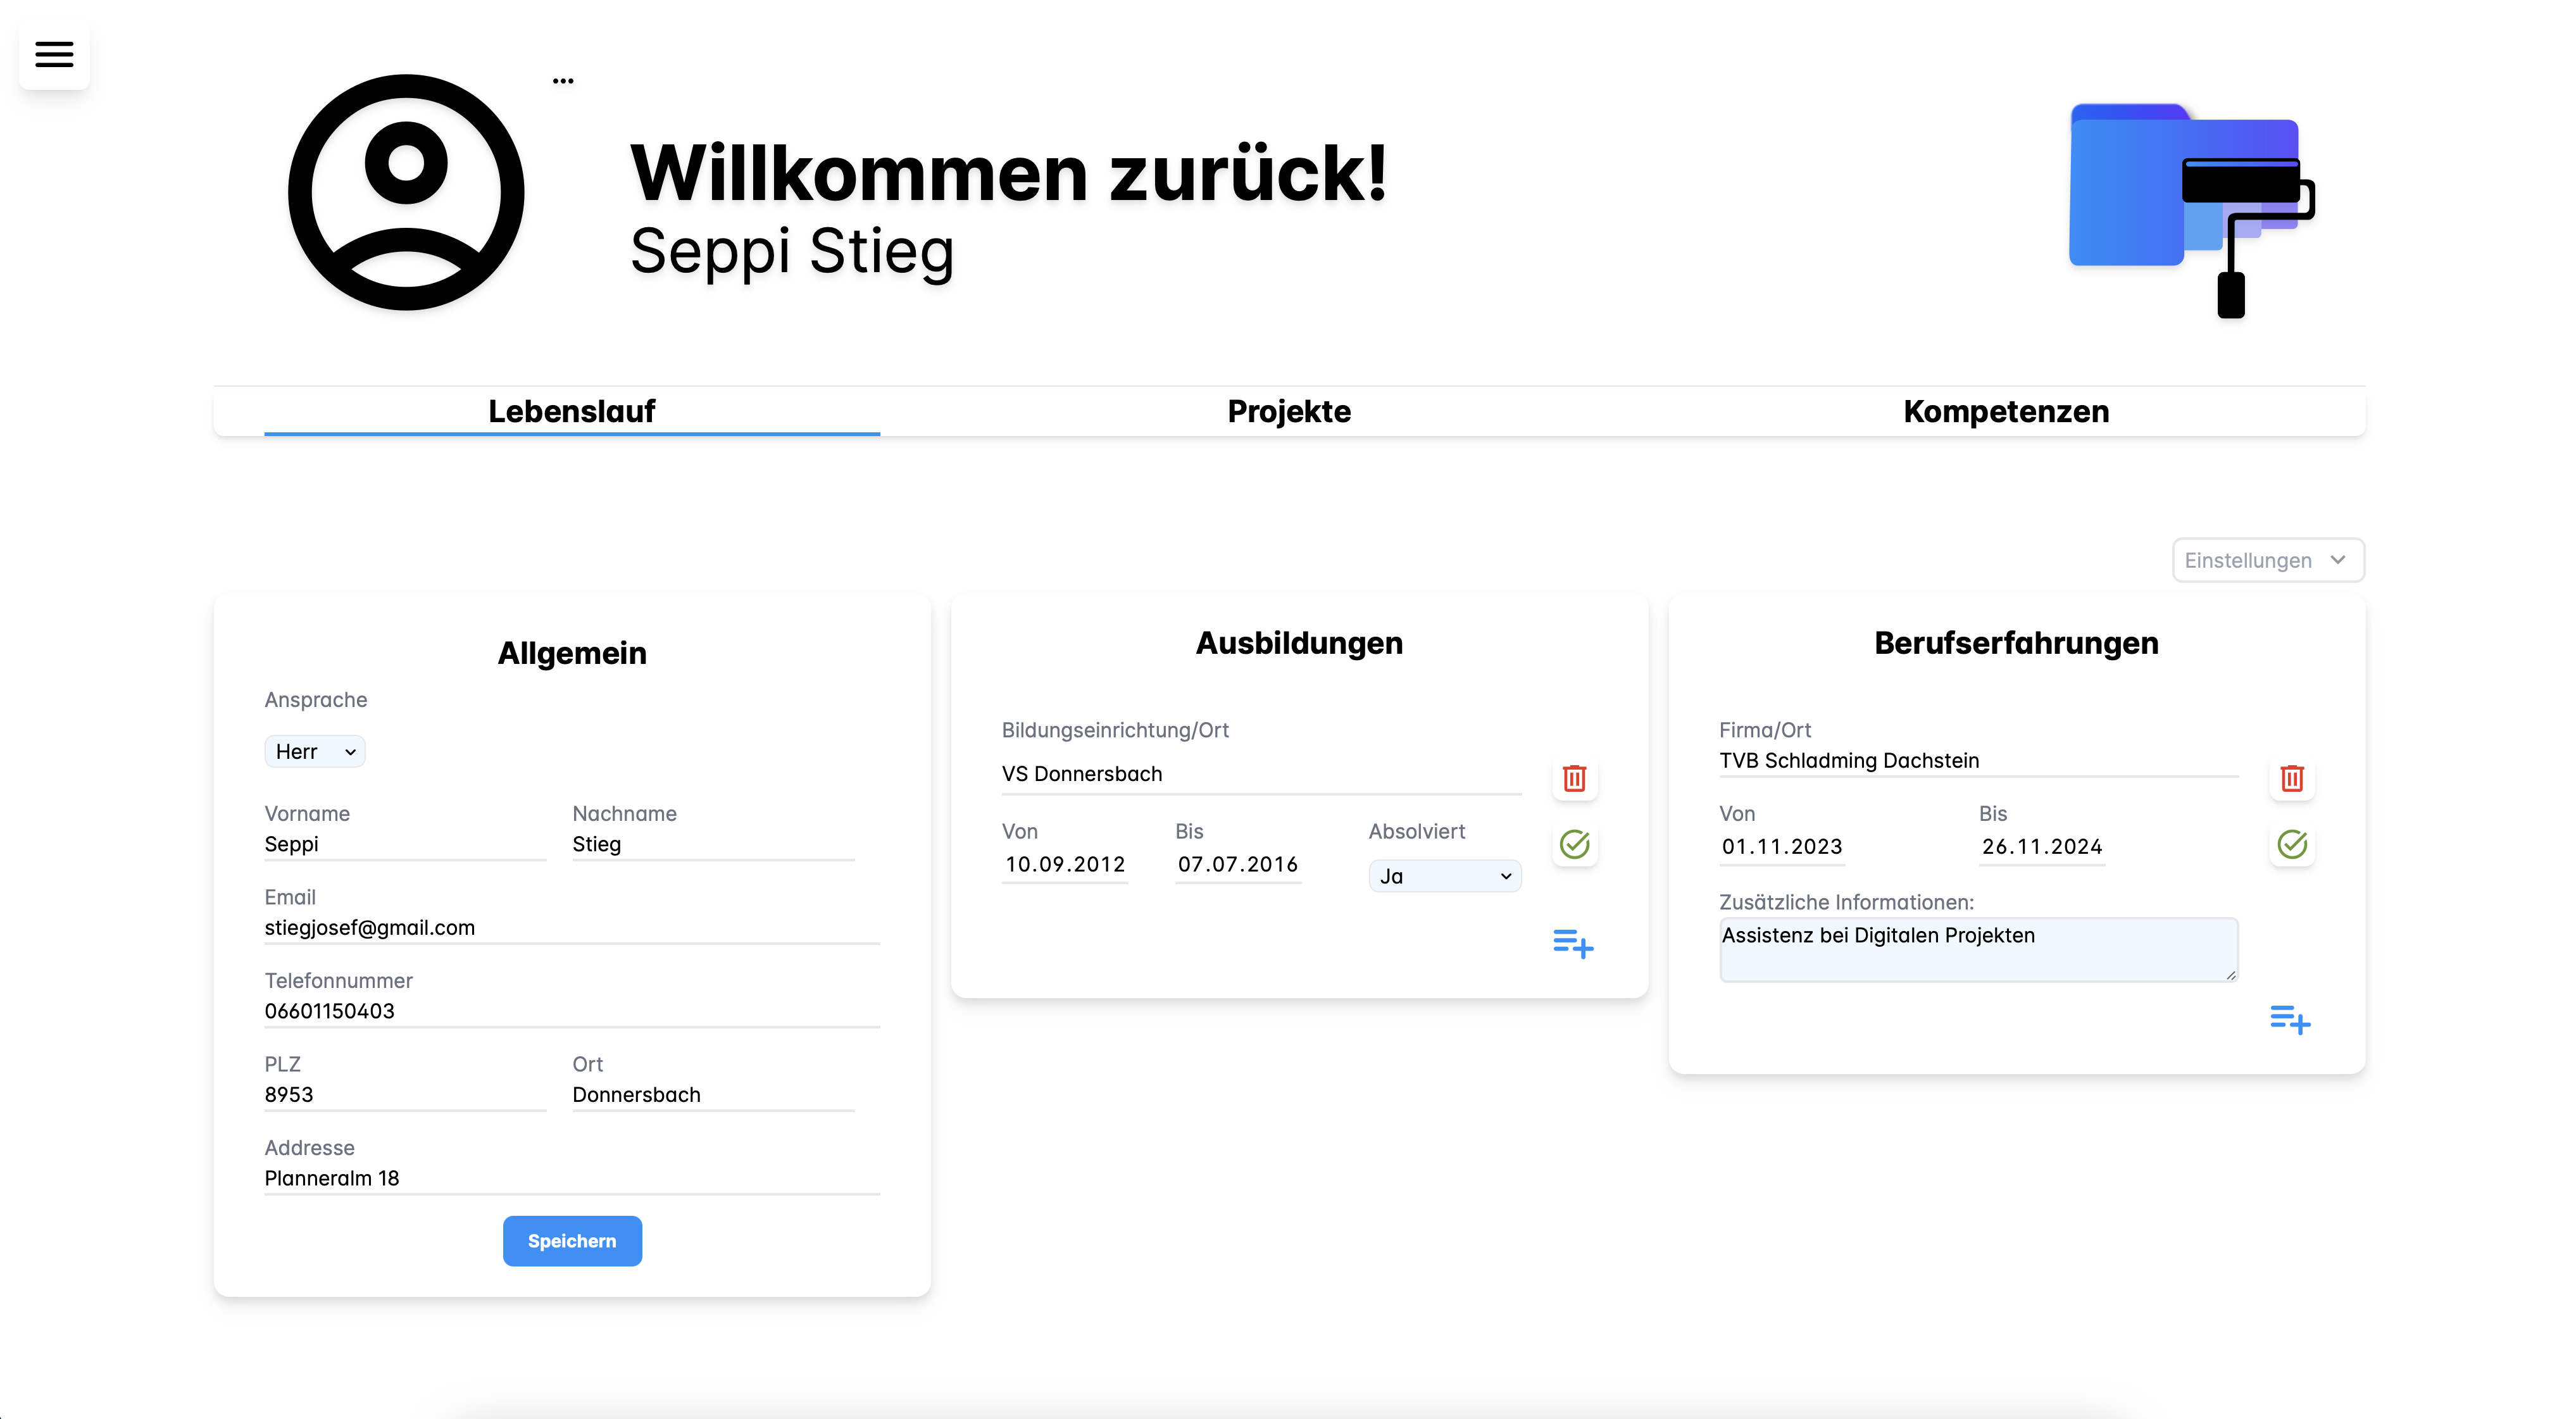
\includegraphics[scale=0.15]{pics/Einführung/Melius_Lebenslauf.png}
    \caption{Abbildung der Melius Home Page}
    \label{fig:int:cv}
\end{figure}

\subsection{Gruppenfunktion}

Neben der Erstellung individueller, personalisierter Portfolios bietet \textit{Melius} eine zusätzliche Funktionalität, die insbesondere auf die Bedürfnisse von Teams, Unternehmen und dem Personalmanagement zugeschnitten ist. Hierbei handelt es sich um die sogenannte "Gruppenfunktion". Die Erweiterung erlaubt die Erstellung, den Beitritt zu sowie die kollaborative Verwaltung von Talenten und Kompetenzen in Gruppen.

Die Gruppenfunktion ist insbesondere darauf ausgerichtet, sowohl die interne Organisation als auch die externe Zusammenarbeit zu erleichtern. Unternehmen, Projektteams oder Organisationen haben die Möglichkeit, Gruppen anzulegen, um alle relevanten Mitglieder, deren Profile und Kompetenzen an einem zentralen Ort zu bündeln. Dies erleichtert nicht nur die Übersicht, sondern auch die gezielte Suche nach spezifischen Fähigkeiten oder Projektanforderungen.

Die Erstellung einer Gruppe ist unkompliziert und anpassungsfähig gestaltet. Administratorinnen und Administratoren sind in der Lage, Gruppen zu definieren und einzuladen, wodurch ein strukturierter Raum für die Mitglieder entsteht. Des Weiteren ist auch der Beitritt zu bereits bestehenden Gruppen mit geringem Aufwand verbunden. Die Registrierung neuer Nutzerinnen und Nutzer sowie die Einladung bereits registrierter Nutzerinnen und Nutzer erfolgt mit nur wenigen Klicks. Dadurch wird es den Nutzerinnen und Nutzern ermöglicht, ihre Profile in den Kontext der Gruppe einzubringen und von einem koordinierten Netzwerk zu profitieren.

Die Gruppenfunktion verfügt über eine besonders nützliche Eigenschaft, nämlich die Möglichkeit, Mitglieder basierend auf ihren Kompetenzen und Qualifikationen zu filtern. Dies erlaubt die selektive Auswahl von Personen, die den Anforderungen eines spezifischen Projekts oder einer bestimmten Aufgabe entsprechen. Beispielsweise kann ein Unternehmen innerhalb der Gruppe nach Mitgliedern mit Kenntnissen in einer bestimmten Programmiersprache, Erfahrung in Projektmanagement-Tools oder anderen spezialisierten Fähigkeiten suchen.
Diese Funktion reduziert den Zeitaufwand für die Suche nach geeigneten Talenten erheblich und gewährleistet die effiziente Nutzung der verfügbaren Ressourcen. Auch bei kurzfristigen Anforderungen kann schnell auf relevante Expertise zurückgegriffen werden.

\begin{figure}[H]
    \centering
    
\includegraphics[scale=0.215]{pics/Einführung/Melius_Gruppen.png}
    \caption{Abbildung der Melius Gruppen Seite}
    \label{fig:int:cv}
\end{figure}

\section{Namensfindung}

Der Name \textit{Melius – The Better Profile} setzt sich aus verschiedenen Namensideen zusammen. Zu Beginn wurde das Projekt lediglich unter der Bezeichnung \textit{Better Profile} geführt. Das Wort \textit{Melius} leitet sich vom lateinischen \textit{Melior} ab, was \textit{besser} bedeutet. Demgemäß würde die lateinische Bezeichnung für \textit{Better Profile, Melius Profile} lauten. Aus der Kombination dieser beiden Elemente entstand schließlich die Bezeichnung \textit{Melius – The Better Profile}.
